\section{Benchmark Variance}
A \nth{3} analysis is done on the Benchmark data to assess the variances of each of the benchmarks evaluated. To achieve this, a single nETL task is run to load a database with Benchmarks data for all students who attended CSC1015F in either 2014, 2015, or 2016 (or attended the course multiple times). The JSON used for configuring nETL to load data from the \texttt{Benchmarks (2014 - 2016).csv} file into CouchDB is included in the appendix at \ref{netl-task-6-config}, which is identical to the configuration of the Task 1 nETL process (except that a different database is used).

Following loading of the data from the CSV into CouchDB, a Map function is used to produce an index of the CouchDB documents sorted by Student ID. Only the single value (Student ID) is used for the key since the Map function only outputs a single document type no joining is required - in fact, since the results of this analysis is the coefficient of variation for each used benchmark, a List function is not required at all. Instead the coefficient of variation of each benchmark analyzed is read directly from the MapReduce output (i.e. the view-index).

\subsection{Map Function}
The map function for this analysis is included in the appendix (see \ref{variance-map-function}). Each document passed to the map function is treated according to the logic shown in the activity diagram in Figure \ref{fig-map-fn-diagram}. ...

That is, on Map function execution the ``type\_'' attribute is checked. If the document is a line of the Grades entity, then the key [Student ID, Course, year] is emitted along with a single number for the value - the percent achieved for the course. If the document is a line of the Benchmarks entity, then the key [student ID, 0, 0] is emitted along with an ordered list of 8 values corresponding to values for the fields in the Benchmarks.CSV file:

\begin{itemize}
    \item Gr12 English \%
    \item Gr12 science \%
    \item Gr12 Math \%
    \item Gr 12 Math Lit \%
    \item Gr12 Adv Math \%
    \item NBT AL \%
    \item NBT QL \%
    \item NBT Math \%
\end{itemize}

Normalization of the percentage fields (i.e. ``Percent'' for the Grades entity and the test results in the Benchmarks entity) is done via a nested function within the Map function and according to the logic as discussed in that tables previously. No reduce function is used to achieve this 2-way join. This is because, theoretically, a student should only have a single set of Benchmark results and should only achieve a single grade per course per year. As such there is no need to aggregate output from the Map function (which is done via reduction) before performing the document join via the List function.

\begin{figure}[ht]
    \centering
    \begin{mdframed}
        \centering
        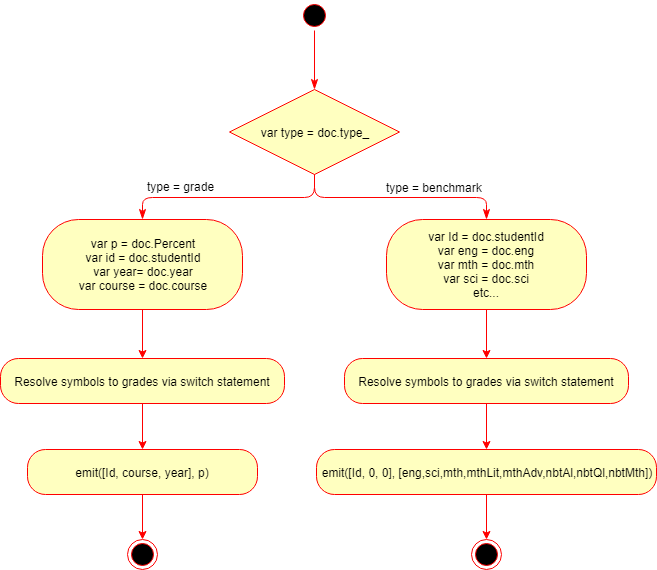
\includegraphics[scale=0.35]{./resources/figures/2-way-join-map.png}
    \end{mdframed}
    \caption[2-Way Join Map Function]{\textbf{Figure \ref{2-way-join-map-fn-diagram}: Map function logic required for the 2-way join.} This logic is applied to every document during index calculation (excluding documents with an \_id of ``\_design/*''). The logic used to normalize grades-as-symbols to percentages is shown in Table \ref{tbl-grades-normalize} for the Grades data, and \ref{tbl-benchmarks-normalize} for the Benchmarks data.}
    \label{2-way-join-map-fn-diagram}
\end{figure}

\subsection{List Function}

\begin{figure}[ht]
    \centering
    \begin{mdframed}
        \centering
        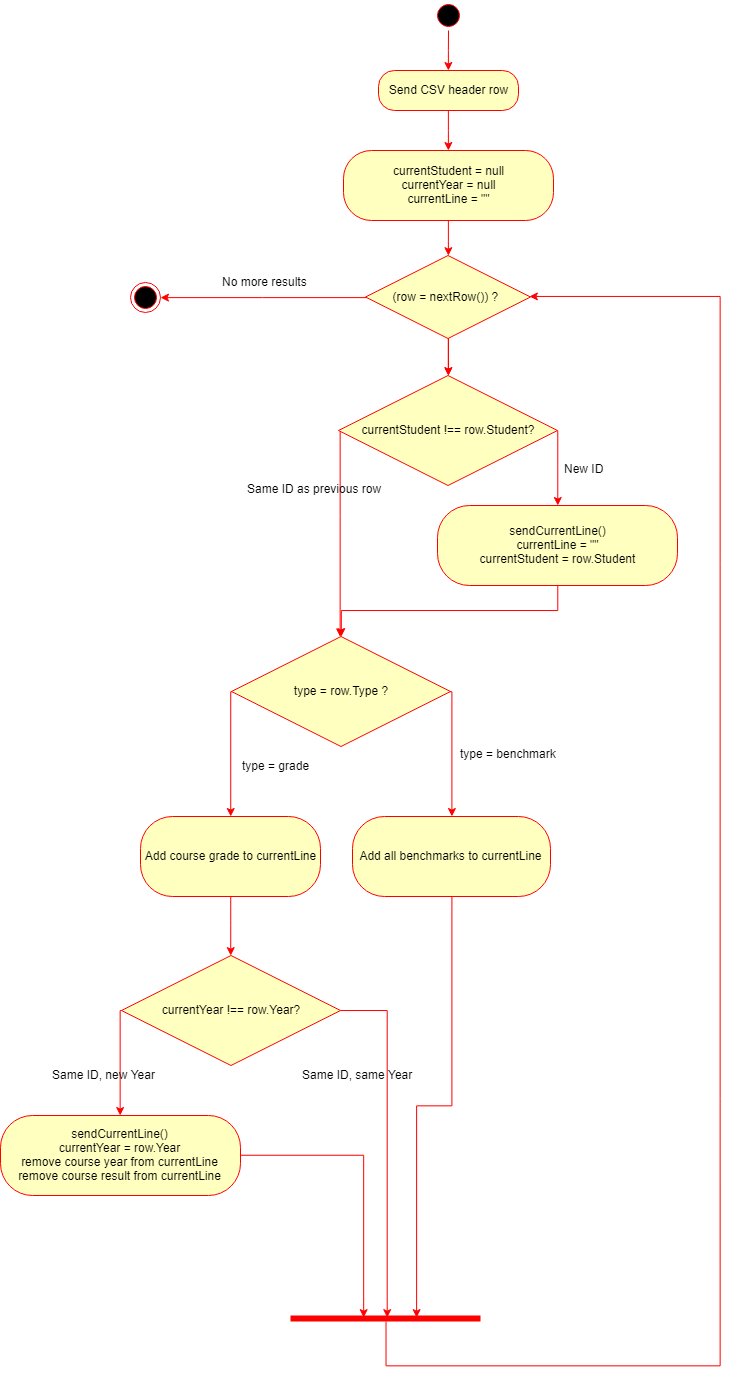
\includegraphics[scale=0.35]{./resources/figures/2-way-join-list.png}
    \end{mdframed}
    \caption[2-Way Join List Function]{\textbf{Figure \ref{fig-2-way-join-list-function}: List function logic required to join the Grades and Benchmarks entities.} Activity diagram of the code executed within the callback passed to the provides function executed by CouchDB during runtime of List function.}
    \label{fig-2-way-join-list-function}
\end{figure}

\subsection{Output}
A sample of the resultant joined dataset is shown in Figure \ref{fig-2-way-csv-output}
\begin{sidewaysfigure}
    \centering
    \begin{mdframed}[rightline=false,topline=false,leftline=false]
        \centering
        \begin{BVerbatim}
+------+---------+----------+-------+---------+---------+---------+-------------+-------------+-------+-------+--------+
| Year |   ID    |  Course  | Grade | G12 Eng | G12 Sci | G12 Mth | G12 Mth Lit | G12 Mth Adv | NBTAL | NBTQL | NBTMth |
+------+---------+----------+-------+---------+---------+---------+-------------+-------------+-------+-------+--------+
| 2015 | 2749802 | CSC1015F |    71 |      79 |      72 |      85 |           0 |           0 |    86 |    94 |     91 |
| 2015 | 2794606 | CSC1015F |    77 |      75 |      84 |      78 |           0 |           0 |     0 |     0 |      0 |
| 2014 | 2854832 | CSC1015F |    87 |      88 |       0 |      97 |           0 |           0 |    81 |    83 |     82 |
| 2014 | 2860166 | CSC1015F |    37 |       0 |       0 |       0 |           0 |           0 |     0 |     0 |      0 |
| 2016 | 2862568 | CSC1015F |    63 |      80 |       0 |      95 |           0 |           0 |    78 |    79 |     82 |
| 2014 | 2863288 | CSC1015F |    81 |      86 |       0 |      93 |           0 |           0 |    82 |    86 |     90 |
| 2015 | 2863336 | CSC1015F |    66 |      71 |      74 |      75 |           0 |           0 |    76 |    78 |     66 |
| 2015 | 2864266 | CSC1015F |    49 |      55 |       0 |      74 |           0 |           0 |    59 |    66 |     61 |
| 2016 | 2864266 | CSC1015F |    64 |      55 |       0 |      74 |           0 |           0 |    59 |    66 |     61 |
| 2014 | 2880284 | CSC1015F |    64 |      68 |       0 |      93 |           0 |           0 |    65 |    92 |     78 |
| 2014 | 2881364 | CSC1015F |    68 |      87 |       0 |      84 |           0 |           0 |    81 |    86 |     73 |
| 2014 | 2882706 | CSC1015F |    85 |      82 |       0 |      97 |           0 |           0 |    83 |    83 |     92 |
| 2014 | 2890964 | CSC1015F |    80 |      74 |       0 |      88 |           0 |           0 |    78 |    88 |     71 |
| 2014 | 2894402 | CSC1015F |    78 |      70 |       0 |      86 |           0 |           0 |    66 |    71 |     70 |
| 2014 | 2894954 | CSC1015F |    87 |      72 |       0 |      94 |           0 |           0 |    81 |    93 |     88 |
| 2014 | 2895244 | CSC1015F |    64 |      77 |       0 |      85 |           0 |           0 |    72 |    54 |     45 |
| 2015 | 2896964 | CSC1015F |    76 |      77 |       0 |      84 |           0 |           0 |    66 |    82 |     71 |
+------+---------+----------+-------+---------+---------+---------+-------------+-------------+-------+-------+--------+
        \end{BVerbatim}
    \end{mdframed}
    \caption[Sample of 2-way CSV output]{\textbf{Figure \ref{fig-2-way-csv-output}: Sample of the 2-way join output CSV.} List function output is a CSV download with the schema as represented in this figure. The full CSV has 1391 rows; 350 rows for the 2014 year, 457 rows for the 2015 year, 586 rows for the 2016 year. Many student IDs are repeated for different years; this occurs when students retake the course in a subsequent year. In this case, due to the nature of the sorted view index from CouchDB, all a student's course attempts are sequential rows.}
    \label{fig-2-way-csv-output}
\end{sidewaysfigure}
